\documentclass[aspectratio=169]{beamer}

\usepackage{tikz}
\usepackage{pgfplots}
\usetheme{default}
\setbeamertemplate{navigation symbols}{}
\setbeamertemplate{itemize item}{\color{black}\textbullet}
\setbeamertemplate{itemize subitem}{\color{black}\textbullet}
\usepackage{xcolor}
\definecolor{navy}{RGB}{0, 0, 128}

\begin{document}

\begin{frame}

Suppose our utility function is given by 
\begin{align*}
X_i\beta_{j} + \gamma_{i}Z_{ij} + \epsilon_{ij}    
\end{align*}

where we assume that $\gamma_i \sim F$ with pdf $f$ and distributional parameters $\mu$ and $\sigma$

\bigskip{}

\onslide<2->{
Then the logit choice probabilities become:

\begin{align*}
P_{ij}\left(X,Z;\beta,\mu,\sigma\right) &= \int\frac{\exp\left(X_{i}\left(\beta_{j}-\beta_{J}\right)+\gamma_i\left(Z_{ij}-Z_{iJ}\right)\right)}{\sum_k \exp\left(X_{i}\left(\beta_{k}-\beta_{J}\right)+\gamma_i\left(Z_{ik}-Z_{iJ}\right)\right)}f\left(\gamma_i;\mu,\sigma\right)d\gamma_i
\end{align*}
}

\end{frame}

\begin{frame}

This is just like the expected value of a function of a random variable $W$:

\onslide<1->{
\begin{align*}
\mathbb{E}[g(W)] &= \int g(W) f\left(W;\mu,\sigma\right)dW
\end{align*}
}

\onslide<2->{
Annoyance: the log likelihood now has an integral inside the log!

{\small
\begin{align*}
\ell\left(X,Z;\beta,\gamma,\mu,\sigma\right) &= \sum_{i=1}^N \log\left\{\int\prod_{j}\left[\frac{\exp\left(X_{i}\left(\beta_{j}-\beta_{J}\right)+\gamma\left(Z_{ij}-Z_{iJ}\right)\right)}{\sum_k \exp\left(X_{i}\left(\beta_{k}-\beta_{J}\right)+\gamma\left(Z_{ik}-Z_{iJ}\right)\right)}\right]^{d_{ij}}f\left(\gamma;\mu,\sigma\right)d\gamma\right\}
\end{align*}
}
}

\onslide<3->{
Can't switch $\log$ and integral because of properties of logarithms
}

\end{frame}

\begin{frame}

Common mixing distributions:
\begin{itemize}
    \item[]<2->
    \item<2-> Normal
    \item[]<3->
    \item<3-> Log-normal
    \item[]<4->
    \item<4-> Uniform
    \item[]<5->
    \item<5-> Triangular
    \item[]<6->
    \item<6-> Can also specify a multivariate normal
    \begin{itemize}
        \item[]<7->
        \item<7-> This would allow, e.g., heterogeneity in $\gamma$ to be correlated with $\beta$
    \end{itemize}
\end{itemize}


\end{frame}

\begin{frame}

With the integral inside the log, estimation of the mixed logit is intensive

\bigskip{}

\onslide<2->{
To estimate the likelihood function, need to numerically approximate the integral
}

\bigskip{}

\onslide<3->{
The most common way of doing this is \textcolor{navy}{quadrature}
}

\bigskip{}

\onslide<4->{
Another common way of doing this is by \textcolor{navy}{simulation} (Monte Carlo integration)
}


\bigskip{}

\onslide<5->{
Choice is often determined by specifics of the problem at hand (e.g. dimensionality)
}

\end{frame}


\begin{frame}

Riemann Sum vs. Quadrature

\bigskip{}

\begin{center}
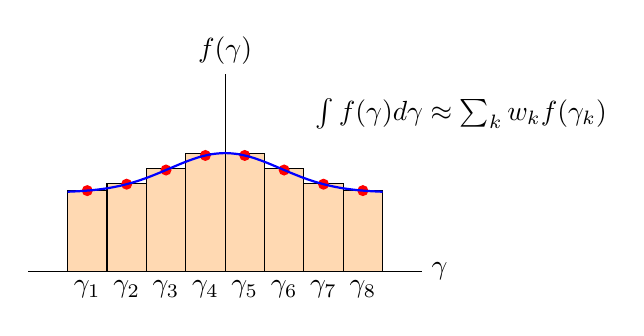
\begin{tikzpicture}
% x-axis
\draw[-] (-2.5,0) -- (2.5,0) node[right] {$\gamma$};
% y-axis  
\draw[-] (0,0) -- (0,2.5) node[above] {$f(\gamma)$};

% Riemann rectangles
\foreach \x in {-2,-1.5,-1,-0.5,0,0.5,1,1.5} {
    \draw[fill=orange!30] (\x,0) rectangle (\x+0.5, {0.5*exp(-\x*\x-0.5*\x) + 1});
}

% Quadrature points
\foreach \x [count=\i] in {-1.75,-1.25,-0.75,-0.25,0.25,0.75,1.25,1.75} {
    \fill[red] (\x, {0.5*exp(-\x*\x) + 1}) circle (2pt);
    \node[below] at (\x,0) {$\gamma_{\i}$};
}

% Weights
\node at (3,2) {$\int f(\gamma) d\gamma \approx \sum_k w_k f(\gamma_k)$};

% Function curve
\draw[thick, blue, overlay] plot[smooth, domain=-2:2] (\x, {0.5*exp(-\x*\x) + 1});

\end{tikzpicture}
\end{center}

\onslide<2->{
\bigskip{}

Riemann sum: $w_k = \Delta \gamma$ for all $k$ (uniform widths)
\bigskip{}

Quadrature: optimal weights $w_k$ (not uniform, chosen for accuracy)
}

\end{frame}


\begin{frame}

Monte Carlo Integration

\bigskip{}

\begin{center}
\begin{tikzpicture}
% x-axis
\draw[-] (-2.5,0) -- (2.5,0) node[right] {$\gamma$};
% y-axis  
\draw[-] (0,0) -- (0,2.5) node[above] {$f(\gamma)$};

% Function curve
\draw[thick, blue] plot[smooth, domain=-2:2] (\x, {0.5*exp(-\x*\x) + 1});

% Random points
\foreach \i in {1,...,50} {
    \pgfmathsetmacro{\x}{4*rand}
    \pgfmathsetmacro{\y}{0.5*exp(-\x*\x) + 1}
    \fill[red] (\x, \y) circle (1pt);
}

% Formula
\node at (3,2) {$\int f(\gamma) d\gamma \approx \frac{1}{R}\sum_{r=1}^R f(\gamma_r)$};
\end{tikzpicture}
\end{center}

\onslide<2->{
\bigskip{}

Monte Carlo: uniform weights $w_r = \frac{1}{R}$ for all random draws

\bigskip{}

Draw $R$ random values $\gamma_r$ from $F\left(\cdot\right)$, take average of function values
}

\onslide<3->{
\bigskip{}

$R$ usually needs to be very large (min. 10,000)
}

\end{frame}


\end{document}